\documentclass{article}
\usepackage[utf8]{inputenc}
\usepackage{amsmath}
\usepackage{amssymb}
\usepackage{geometry}
\usepackage{graphicx}
\usepackage{float}
\usepackage{tikz}
\usetikzlibrary{shapes.geometric, arrows, positioning, calc, patterns}

\geometry{a4paper, margin=1in}

\title{Model Extension: Author-Journal Game with Competition and Capacity Constraints}

\date{\today}

\begin{document}

\maketitle

\section{Motivation and Problem Statement}

In our previous evolutionary game-theoretic model of the author-journal interaction, we observed that the equilibrium strategies were largely insensitive to the population size $N$. This phenomenon arises because, in the original formulation, the payoff of a focal author depends solely on their own strategy and the journal's acceptance policy, but is independent of the actions of other authors. Consequently, there is no \textit{congestion effect} or \textit{competition} for limited resources.

To address this and model a more realistic academic publishing environment (e.g., conferences with fixed acceptance rates or journals with limited pages), we introduce a capacity threshold $K$. This mechanism creates a zero-sum element: as the number of submissions increases, the probability of acceptance for a passed paper decreases, potentially disincentivizing opportunistic strategies like \textit{Always Submit} (AS).

\section{The Threshold Competition Model}


The updated interaction proceeds in the following stages:
\begin{enumerate}
    \item \textbf{Submission:} $N$ authors choose a strategy $s \in \{OG, AS, \dots\}$.
    \item \textbf{Peer Review (Perception):} All submissions undergo peer review characterized by false negative rate $\epsilon$ and false positive rate $\lambda$. Papers that pass peer review enter a ``Perception Pool'' of size $M$.
    \item \textbf{Competition (Threshold Cut):} The journal has a maximum capacity $K$.
    \begin{itemize}
        \item If $M \le K$, all papers in the pool are accepted.
        \item If $M > K$, the journal randomly selects $K$ papers from the pool to accept. The remaining $M-K$ papers are rejected despite passing review.
    \end{itemize}
\end{enumerate}


Let $\alpha$ be the probability an author produces a good paper. The probability that a single author's submission passes the peer review stage, denoted as $P_{pass}(s)$, depends on their chosen strategy $s$:

\begin{align}
    P_{pass}(OG) &= \alpha(1-\epsilon) \\
    P_{pass}(AS) &= \alpha(1-\epsilon) + (1-\alpha)\lambda
\end{align}

Here, $OG$ authors only submit good papers, while $AS$ authors submit both good and bad papers, benefiting from the false positive rate $\lambda$.


\begin{figure}[htbp]
    \centering
    % 这一行让图片自动缩放适应页面宽度
    \resizebox{\textwidth}{!}{
        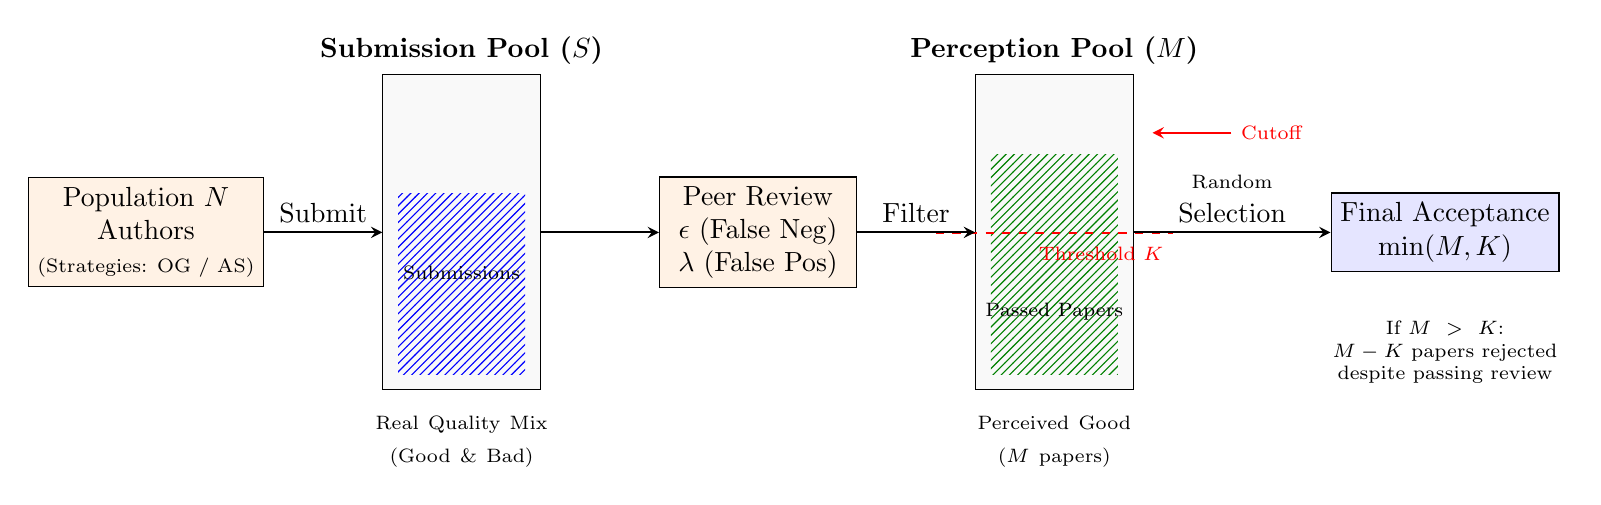
\begin{tikzpicture}[node distance=2cm, auto, >=stealth]

        % --- 定义样式 ---
        \tikzstyle{process} = [rectangle, minimum width=2.5cm, minimum height=1cm, text centered, draw=black, fill=orange!10]
        \tikzstyle{pool} = [rectangle, minimum width=2cm, minimum height=4cm, draw=black, fill=gray!5]
        \tikzstyle{arrow} = [thick,->]

        % --- 节点定义 ---

        % 1. Authors
        \node (authors) [process, align=center] {Population $N$ \\ Authors \\ \scriptsize (Strategies: OG / AS)};

        % 2. Submission Pool
        \node (submit_pool) [pool, right=1.5cm of authors, label=above:\textbf{Submission Pool ($S$)}] {};
        \fill[pattern=north east lines, pattern color=blue] ($(submit_pool.south west) + (0.2,0.2)$) rectangle ($(submit_pool.south east) + (-0.2, 2.5)$);
        \node at ($(submit_pool.south) + (0, 1.5)$) {\scriptsize Submissions};

        % 3. Peer Review
        \node (review) [process, right=1.5cm of submit_pool, align=center] {Peer Review \\ $\epsilon$ (False Neg) \\ $\lambda$ (False Pos)};

        % 4. Perception Pool
        \node (percep_pool) [pool, right=1.5cm of review, label=above:\textbf{Perception Pool ($M$)}] {};
        \fill[pattern=north east lines, pattern color=green!50!black] ($(percep_pool.south west) + (0.2,0.2)$) rectangle ($(percep_pool.south east) + (-0.2, 3.0)$);
        \node at ($(percep_pool.south) + (0, 1.0)$) {\scriptsize Passed Papers};

        % --- Threshold K (红色虚线与文字) ---
        \draw[red, thick, dashed] ($(percep_pool.south west) + (-0.5, 2.0)$) -- ($(percep_pool.south east) + (0.5, 2.0)$);
        % 文字在虚线右下方
        \node[text=red, anchor=north east, yshift=-0.05cm] at ($(percep_pool.south east) + (0.5, 2.0)$) {\scriptsize Threshold $K$};

        % 5. Final Selection
        \node (final) [process, right=2.5cm of percep_pool, align=center, fill=blue!10] {Final Acceptance \\ $\min(M, K)$};

        % --- 连线 ---
        \draw[arrow] (authors) -- node[above] {Submit} (submit_pool);
        \draw[arrow] (submit_pool) -- (review);
        \draw[arrow] (review) -- node[above] {Filter} (percep_pool);

        % --- Cutoff (Cutoff 在 Random Selection 上方,箭头向左) ---
        \draw[arrow] (percep_pool) -- node[above, align=center] (rand_sel) {\scriptsize Random\\Selection} (final);
        
        % Label
        \node[above=0.2cm of rand_sel, xshift=0.5cm, text=red] (cutoff_label) {\scriptsize Cutoff};
        % Arrow pointing LEFT
        \draw[->, red, thick] (cutoff_label.west) -- ++(-1.0, 0);

        % --- 底部注释 ---
        \node [below=0.2cm of submit_pool, text width=2.5cm, align=center] {\scriptsize Real Quality Mix\\(Good \& Bad)};
        \node [below=0.2cm of percep_pool, text width=2.5cm, align=center] {\scriptsize Perceived Good\\($M$ papers)};
        \node [below=0.5cm of final, text width=3cm, align=center, font=\scriptsize] {If $M > K$: \\ $M-K$ papers rejected \\ despite passing review};

        \end{tikzpicture}
    }
    \caption{\textbf{Schematic representation of the Threshold Competition Model.} The process unfolds in three stages: (1) Submission into a pool $S$; (2) Peer review filtering into a perception pool $M$; and (3) A hard capacity constraint $K$ (red dashed line). If $M > K$, a random cutoff occurs, rejecting surplus papers even if they passed review. This introduces the competition factor $\gamma$.}
    \label{fig:threshold_model}
\end{figure}
\section{Derivation of the Competition Factor $\gamma$}

The key addition to the payoff function is the competition factor $\gamma$, which represents the probability that a paper is finally accepted \textit{given that it has already passed peer review}.

Let us consider a \textit{focal author} who has passed peer review. Let $M_{-i}$ be the random variable representing the number of \textit{other} authors (out of $N-1$) whose papers also passed peer review.

The total number of passed papers is therefore $M = 1 + M_{-i}$.

The competition factor for the focal author is defined as:
\begin{equation}
    \gamma_{\text{focal}} = \min\left(1, \frac{K}{1 + M_{-i}}\right) = 
    \begin{cases} 
      1 & \text{if } 1 + M_{-i} \le K \\
      \frac{K}{1 + M_{-i}} & \text{if } 1 + M_{-i} > K
   \end{cases}
\end{equation}

\subsection{Expected Competition Factor}
Since $M_{-i}$ is a random variable, authors base their decisions on the expected value $E[\gamma_{\text{focal}}]$. 

Assume the population consists of $N_{OG}$ authors playing $OG$ and $N_{AS}$ authors playing $AS$ (where $N_{OG} + N_{AS} = N - 1$, excluding the focal author). The variable $M_{-i}$ is the sum of two independent binomial distributions:
\begin{equation}
    M_{-i} = X_{OG} + X_{AS}
\end{equation}
where $X_{OG} \sim B(N_{OG}, P_{pass}(OG))$ and $X_{AS} \sim B(N_{AS}, P_{pass}(AS))$.

The expected competition factor is given by:
\begin{equation}
    E[\gamma_{\text{focal}}] = \sum_{m=0}^{N-1} \Pr(M_{-i} = m) \cdot \min\left(1, \frac{K}{1 + m}\right)
\end{equation}

\section{Updated Payoff Functions}

We incorporate $E[\gamma_{\text{focal}}]$ into the utility functions. Let $r$ be the reward for acceptance and $c$ be the cost of submission.


An $OG$ author submits with probability $\alpha$. If they submit, they pay cost $c$. They pass review with probability $1-\epsilon$. If they pass, they are accepted with probability $E[\gamma_{\text{focal}}]$.

\begin{equation}
    U_A(OG) = \alpha \left[ (1-\epsilon) \cdot E[\gamma_{\text{focal}}] \cdot r - c \right]
\end{equation}
\textit{Note: Assuming cost is paid per submission regardless of acceptance.}


An $AS$ author always submits (probability 1), paying cost $c$. They pass review with probability $P_{pass}(AS)$. If they pass, they are accepted with probability $E[\gamma_{\text{focal}}]$.

\begin{equation}
    U_A(AS) = \left[ (\alpha(1-\epsilon) + (1-\alpha)\lambda) \cdot E[\gamma_{\text{focal}}] \cdot r \right] - c
\end{equation}


The journal's utility depends on the quality of the final accepted papers and the cost of reviewing the total volume of submissions. 

Let $B$ be the benefit for accepting a good paper and $D$ be the penalty for accepting a bad paper.
The total submission volume $S$ is given by:
\begin{equation}
    E[S] = N_{OG} \cdot \alpha + N_{AS} \cdot 1
\end{equation}

The ``Perception Pool'' $M$ contains a mix of good and bad papers that passed review.
The expected number of good papers ($M_G$) and bad papers ($M_B$) in the pool are:
\begin{align}
    E[M_G] &= (N_{OG} + N_{AS}) \cdot \alpha(1-\epsilon) \\
    E[M_B] &= N_{AS} \cdot (1-\alpha)\lambda
\end{align}
\textit{Note: Both OG and AS authors contribute to $M_G$, but only AS authors contribute to $M_B$.}

Since the journal selects $K$ papers randomly from $M$ (if $M > K$), the final accepted papers maintain the same quality ratio as the pool. The expected acceptance rate for any paper in the pool is approximated by the system-wide competition factor $\bar{\gamma} = E[\min(1, K/M)]$.

The journal's expected payoff is:
\begin{equation}
    U_J = B \cdot (E[M_G] \cdot \bar{\gamma}) - D \cdot (E[M_B] \cdot \bar{\gamma}) - C(E[S])
\end{equation}

Where $C(S)$ is the cost function (e.g., linear or convex with respect to total submissions). This formulation highlights that while $K$ limits the absolute number of bad papers accepted (by reducing $\bar{\gamma}$), it does not improve the \textit{ratio} of good to bad papers, which is still determined by $\epsilon$ and $\lambda$.
\section{Discussion: The Effect of $N$}

In this new model, the population size $N$ plays a decisive role in shaping equilibrium outcomes, particularly when the journal's capacity $K$ remains fixed or grows at a slower rate than $N$. As the number of authors increases, the expected number of papers passing peer review, $E[M]$, naturally rises. This effect is exacerbated if authors adopt the \textit{Always Submit} (AS) strategy, which floods the perception pool with bad papers that pass due to the false positive rate $\lambda$. This surge in submissions shifts the probability distribution of $M_{-i}$ toward higher values, thereby mechanically reducing the expected competition factor $E[\gamma_{\text{focal}}]$. Consequently, the effective reward for publication is diluted. If $E[\gamma_{\text{focal}}]$ drops below a critical threshold, the expected benefit of the indiscriminate $AS$ strategy may no longer cover the submission cost $c$. This mechanism creates a congestion effect that can potentially restore the stability of the cooperative \textit{Only Good} (OG) strategy or, in extreme cases of overcrowding, lead to a \textit{No Submit} (NS) equilibrium. Thus, the model effectively reintroduces the ``tragedy of the commons,'' demonstrating that population size and finite resource constraints are fundamental determinants of stability in the academic publishing ecosystem.

\section{Determination of Capacity $K$}

The parameter $K$ represents the scarcity of resources (e.g., journal pages or conference presentation slots). To ensure the model reflects realistic dynamics, we propose determining $K$ through two complementary approaches: empirical anchoring and regime analysis.


We can calibrate $K$ based on historical data from top-tier venues. For instance, top computer science conferences (such as ICLR) typically maintain an acceptance rate between 20\% and 30\%. Therefore, in our simulations, we can anchor $K$ such that:
\begin{equation}
    K \approx \delta \cdot N, \quad \text{where } \delta \in [0.2, 0.3]
\end{equation}
This ensures the baseline competition level matches real-world observations.


To fully explore the strategic implications of competition, we analyze the model across three distinct capacity regimes:

\begin{itemize}
    \item \textbf{Resource Scarcity ($K \ll \alpha N$):} In this regime (e.g., $K \approx 0.1N$), competition is intense. The value of $\gamma$ is significantly less than 1 even if all authors cooperate (play OG). Here, the primary driver is the raw capacity constraint, which may force authors into $NS$ strategies to avoid sunk costs.
    
    \item \textbf{Balanced Resources ($K \approx \alpha N$):} This is the most strategically critical regime. The capacity is sufficient to accommodate most good papers, provided authors do not flood the system with bad ones. However, if a significant fraction of authors switches to $AS$, the system quickly becomes congested, causing $\gamma$ to drop. This regime highlights the tension between individual opportunism and collective efficiency.
    
    \item \textbf{Resource Abundance ($K \to N$):} When capacity is abundant (e.g., $K \ge 0.8N$), the competition factor $\gamma \to 1$. In this limit, the model converges back to our original formulation without the threshold constraint, serving as a control group to isolate the effects of competition.
\end{itemize}

\section{Simulation Analysis and Discussion}

Based on the theoretical framework of the Threshold Competition Model, we conducted numerical simulations to examine how the capacity constraint ($K$) and population size ($N$) shape strategic outcomes for authors and journals. This section summarises the simulation design and discusses the main qualitative patterns that emerge.

The simulation environment is constructed as a ``funnel selection'' process, mirroring the constraints of top-tier conferences. Unless stated otherwise, we use $N=100$, $K=20$, $\epsilon=\lambda=0.1$, $B=1.0$, and $D=3.0$. These values implement the following design choices:
\begin{itemize}
    \item \textbf{Funnel mechanism:} The process has three stages: a \emph{Submission Pool} ($S$) generated by $N$ authors; a \emph{Perception Pool} ($M$) filtered by noisy peer review; and a final \emph{Threshold Cut} in which at most $K$ papers are accepted.
    \item \textbf{Resource scarcity:} With $N=100$ and $K=20$, the baseline acceptance rate is only 20\%, creating intense competition for limited slots.
    \item \textbf{Peer-review noise:} Reviewers misclassify good and bad papers with probability $0.1$, providing a niche for the \textit{Always Submit} (AS) strategy to exploit false positives.
    \item \textbf{High penalty for bad papers:} The journal incurs a much larger loss for publishing a bad paper than it gains from a good one ($D>B$), capturing the incentives of reputation-sensitive venues.
\end{itemize}

To maintain mathematical control, we avoid Monte Carlo sampling and instead use two deterministic components:
\begin{enumerate}
    \item \textbf{Exact probability convolution.} For a given mixture of cooperative (OG) and opportunistic (AS) authors, the distribution of the number of passing papers $M_{-i}$ contributed by the rest of the population is obtained as the convolution of two binomial distributions. This yields an exact value for the expected competition factor $E[\gamma]$.
    \item \textbf{Coupled replicator dynamics.} Author strategies evolve according to the expected payoffs determined by $E[\gamma]$, while journal strategies simultaneously adapt their selectivity ($\phi_{OG}$) based on the expected quality of the accepted pool.
\end{enumerate}

\subsection{Static Analysis: Congestion and the Commons}

Figure~\ref{fig:static_analysis} presents the static analysis of the competition factor $E[\gamma]$, isolating the effects of strategy mix and population size.

\begin{figure}[htbp]
    \centering
    % 请确保使用静态分析图的文件名
    \includegraphics[width=\textwidth]{static_analysis.png}
    \caption{\textbf{Static analysis of competition.} \textbf{Left:} Decline of $E[\gamma]$ as the proportion of AS authors increases ($N=100$, $K=20$), illustrating a tragedy-of-the-commons effect. \textbf{Right:} Dependence of $E[\gamma]$ on population size $N$ (with $K=20$), highlighting the onset of congestion.}
    \label{fig:static_analysis}
\end{figure}

The right panel resolves the earlier anomaly that payoffs appeared insensitive to $N$ in simpler models. For small populations ($N\lesssim 40$), the expected number of passing papers remains below the capacity $K$, so $E[\gamma]=1$ and the capacity constraint is non-binding. In this pre-congestion regime, enlarging the population does not affect individual acceptance probabilities, which explains why purely linear models fail to detect any $N$-dependence. Once $N$ crosses the approximate saturation threshold $N \approx K / P_{pass}$, the system enters a congestion regime in which $E[\gamma]$ falls sharply towards $K/M \approx 0.2$. The threshold $K$ thus acts as a critical link between macroscopic population size and microscopic strategic payoffs.

The left panel shows how opportunism feeds back on itself. As the share of AS authors increases, both genuine contributions and false positives inflate the perception pool $M$. Because only $K$ papers can be accepted, the per-paper competition factor $\gamma = K/M$ shrinks for everyone. Individually profitable deviations towards AS therefore generate a tragedy-of-the-commons outcome at the population level.

\subsection{Co-evolutionary Dynamics}

Figure~\ref{fig:dynamic_evolution} turns to the full co-evolutionary dynamics of authors and journals.

\begin{figure}[htbp]
    \centering
    % 请确保使用动态演化图的文件名 (包含时间序列的那张)
    \includegraphics[width=\textwidth]{dynamic_evolution.png}
    \caption{\textbf{Co-evolutionary dynamics.} \textbf{Left:} Time series of the share of AS authors ($\theta_{AS}$, blue) and OG journals ($\phi_{OG}$, red dashed). \textbf{Right:} Phase-plane trajectory showing the specific evolution from the initial state $(\theta_{AS}=0.5, \phi_{OG}=0.5)$.}
    \label{fig:dynamic_evolution}
\end{figure}

The time series (left panel) reveals a clear separation of time scales. The journal population reacts almost instantly: under high penalties for bad publications and strong congestion ($K=20$), the \textit{Always Accept} policy becomes prohibitively costly, and journals rapidly converge to strict selection ($\phi_{OG}\approx 1$). By contrast, authors adapt more slowly. Starting from $\theta_{AS}=0.5$, the share of opportunistic authors gradually declines towards $\theta_{AS}\approx 0.2$ as AS becomes doubly penalised: first by strict peer review (via $\epsilon$), and second by the reduced competition factor ($\gamma<1$) caused by congestion.

\subsection{Global Stability and Robustness}

To ensure the observed outcome is robust to initial conditions, Figure~\ref{fig:phase_plane_global} provides a global view of the system's dynamics using a detailed phase plane.

\begin{figure}[htbp]
    \centering
    % 请插入那张带有灰色流线和多条彩色轨迹的图
    % 建议重命名为 phase_plane_global.png
    \includegraphics[width=0.85\textwidth]{phase_plane_global.png}
    \caption{\textbf{Global stability analysis.} Phase-plane trajectories in the $(\theta_{AS},\phi_{OG})$ plane starting from various initial conditions (coloured lines). Grey streamlines represent the evolutionary vector field, indicating the direction of drift under replicator dynamics.}
    \label{fig:phase_plane_global}
\end{figure}

The horizontal axis represents the authors' behaviour (from fully cooperative on the left to fully opportunistic on the right); the vertical axis represents journal policy (from permissive at the bottom to strict at the top). Grey streamlines act as ``evolutionary currents,'' indicating the system's inherent drive at any given state.

Across all starting points, trajectories display a characteristic inverted ``L'' shape. They first move almost vertically upward as journals swiftly adopt strict screening, and only then drift horizontally leftwards as authors slowly abandon the AS strategy. This asymmetry confirms that institutions act as the \emph{fast variable}, while cultural adaptation among authors is the \emph{slow variable}. 

Crucially, all trajectories converge to the top-left region of the phase plane, characterised by high journal selectivity and a low prevalence of opportunistic submission. This global convergence demonstrates the robustness of the threshold mechanism: once capacity constraints and penalties for bad papers are strong enough, journals are forced to establish credible quality control, and authors subsequently evolve towards high-effort, high-quality behaviour. Institutions must therefore lead so that culture can follow; cooperative norms among authors emerge as a consequence of credible, resource-constrained screening rather than as an exogenous assumption.



\end{document}



